\documentclass[convert={density=300,size=1080x800,outext=.png}]{standalone}
\usepackage{xcolor}
\usepackage{graphics, graphicx}
\usepackage{tikz, tkz-graph}
\usepackage{pgf, pgfplots}
\usepackage{graphviz, tkz-berge}
\usepackage{graphics, graphicx}
\usepackage{pstricks, pst-node, pst-tree}

\usetikzlibrary{arrows, petri, topaths}
\usetikzlibrary{shapes}
\usetikzlibrary{arrows.meta}
\usetikzlibrary{positioning,automata}



\begin{document}
		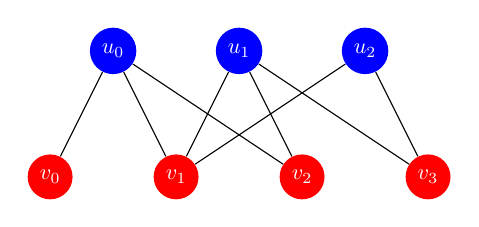
\begin{tikzpicture}[v/.style={circle, fill=red, text=white, thin, minimum size=.5mm}, u/.style={circle, fill=blue, text=white, thin, minimum size=.5mm}, transform shape, scale=0.80]
		\node[v] (a) at (0,0){$v_{0}$};
		\node[v] (b) at (2,0){$v_{1}$};
		\node[v] (c) at (4,0){$v_{2}$};
		\node[v] (d) at (6,0){$v_{3}$};
		\node[u] (e) at (1,2){$u_{0}$};
		\node[u] (f) at (3,2){$u_{1}$};
		\node[u] (g) at (5,2){$u_{2}$};
		\draw (a) edge (e);
		\draw (b) edge (e);
		\draw (b) edge (f);
		\draw (b) edge (g);
		\draw (c) edge (e);
		\draw (c) edge (f);
		\draw (d) edge (f);
		\draw (d) edge (g);
		\end{tikzpicture}
\end{document}